\documentclass{standalone}
\usepackage{amsmath}
\usepackage{amssymb}
\usepackage{tikz}
\usepackage{mathrsfs}
\usepackage{ifthen}

\newcommand{\perpp}{\perp\!\!\!\perp}
\DeclareMathOperator{\so}{\mathfrak{s}}
\DeclareMathOperator{\ra}{\mathfrak{r}}
\DeclareMathOperator{\supp}{supp}
\DeclareMathOperator{\id}{id}
\DeclareMathOperator{\dom}{dom}
\DeclareMathOperator{\ran}{ran}
\DeclareMathOperator{\Min}{Min}
\DeclareMathOperator{\cod}{cod}
\newcommand{\smallerthan}{<}
\newcommand{\greaterthan}{>}
\newcommand{\defeq}{:=}
\newcommand{\eqdef}{=:}

\newcommand{\cat}[1]{\textbf{#1}}
\DeclareMathOperator{\IG}{\mathscr{IG}}


\begin{document}
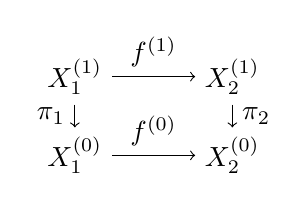
\begin{tikzpicture}
\node (X11) at (0,0) {$X_1^{(1)}$};
\node (X10) at ([shift={+(0,-1)}]X11) {$X_1^{(0)}$};
\node (X21) at ([shift={+(2,0)}]X11) {$X_2^{(1)}$};
\node (X20) at ([shift={+(0,-1)}]X21) {$X_2^{(0)}$};
\draw[->] (X11)--(X21) node[midway,above] {$f^{(1)}$};
\draw[->] (X11)--(X10) node[midway,left] {$\pi_1$};
\draw[->] (X21)--(X20) node[midway,right] {$\pi_2$};
\draw[->] (X10)--(X20) node[midway,above] {$f^{(0)}$};
\end{tikzpicture}\end{document}